% !TeX program = xelatex
\documentclass{article}
\usepackage{xeCJK}
\usepackage{tikz}
\usepackage[outline]{contour}
\usepackage{graphicx}
\graphicspath{ {./} }
\setCJKmainfont{Kaiti SC}
% \setCJKmainfont{Xingkai SC}
% \setCJKmainfont{STKaiti}

\newcommand\Grid[1]{%
 \tikz[baseline=(char.base)]{%
  \draw[xstep=1ex,ystep=1ex,help lines] (-1ex,-1ex) grid (1ex,1ex);
  \draw[help lines,densely dash dot]
  (-1ex,-1ex) -- (1ex,1ex)  (-1ex,1ex) -- (1ex,-1ex);
  \node[inner sep=0pt] (char) at (0,0) {#1};
 }%
}
\pagenumbering{gobble}
\begin{document}
\begin{center}
    \Huge 长歌行 \\
\end{center}
\begin{flushright}
    \huge 汉 $\bullet$ 汉乐府 \\
\end{flushright}
\begin{center}
    \Huge 青青园中葵 \\
    \Huge 朝露待日晞 \\
    \Huge 阳春布德泽 \\
    \Huge 万物生光辉 \\
    \Huge 常恐秋节至 \\
    \Huge 焜黄华叶衰 \\
    \Huge 百川东到海 \\
    \Huge 何时复西归 \\
    \Huge 少壮不努力 \\
    \Huge 老大徒伤悲 \\
\end{center}
\hrule
\begin{center}
    \Huge \Grid{长}\Grid{歌}\Grid{行} \\
\end{center}
\begin{flushright}
    \huge \Grid{汉} $\bullet$ \Grid{汉}\Grid{乐}\Grid{府} \\
\end{flushright}
\begin{center}
    \Huge \Grid{青}\Grid{青}\Grid{园}\Grid{中}\Grid{葵} \\
    \Huge \Grid{朝}\Grid{露}\Grid{待}\Grid{日}\Grid{晞} \\
    \Huge \Grid{阳}\Grid{春}\Grid{布}\Grid{德}\Grid{泽} \\
    \Huge \Grid{万}\Grid{物}\Grid{生}\Grid{光}\Grid{辉} \\
    \Huge \Grid{常}\Grid{恐}\Grid{秋}\Grid{节}\Grid{至} \\
    \Huge \Grid{焜}\Grid{黄}\Grid{华}\Grid{叶}\Grid{衰} \\
    \Huge \Grid{百}\Grid{川}\Grid{东}\Grid{到}\Grid{海} \\
    \Huge \Grid{何}\Grid{时}\Grid{复}\Grid{西}\Grid{归} \\
    \Huge \Grid{少}\Grid{壮}\Grid{不}\Grid{努}\Grid{力} \\
    \Huge \Grid{老}\Grid{大}\Grid{徒}\Grid{伤}\Grid{悲} \\
\end{center}
\hrule
\newpage
\begin{figure}
    \centering
    \makebox[0pt]{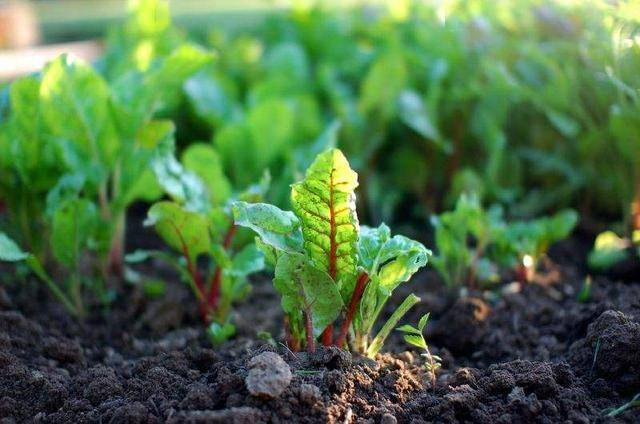
\includegraphics[width=0.9\paperwidth]{fa0a09a992cf43beabd3f900e01f65f3.jpeg}}
\end{figure}
\end{document}
